% Standalone source of the figure fig:kernel of the continuum-limit paper.
% Build: pdflatex fig_kernel.tex; the paper includes the PDF.
\documentclass[border=2pt]{standalone}
% Shared preamble of the continuum-limit paper's standalone figures.
\usepackage{amsmath,amssymb,bm}
\usepackage{tikz}
\usetikzlibrary{calc}
\newcommand{\bS}{\mathbf{S}}
\newcommand{\bG}{\mathbf{G}}
\newcommand{\bK}{\mathbf{K}}
\newcommand{\bP}{\mathbf{P}}
\newcommand{\sinc}{\operatorname{sinc}}

\begin{document}
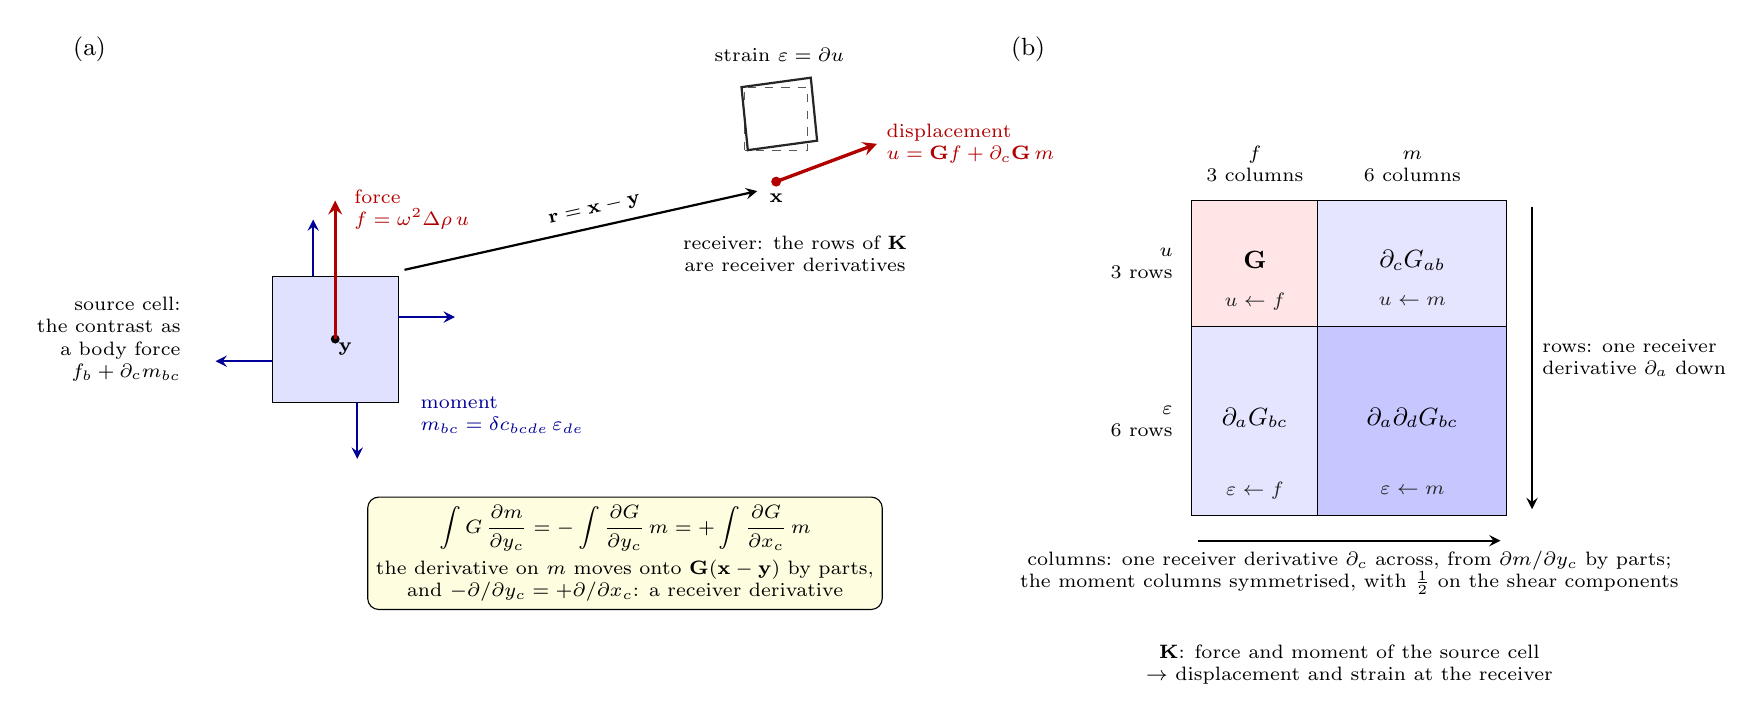
\begin{tikzpicture}[>=stealth, x=0.8cm, y=0.8cm, font=\small]
  % (a) the source cell radiates by a force and a moment; the receiver records displacement and strain
  \begin{scope}
    \node at (-3.9,4.6) {(a)};
    % source cell
    \draw[fill=blue!12] (-1,-1) rectangle (1,1);
    \fill (0,0) circle (1.6pt);
    \node[below right, font=\scriptsize, inner sep=1pt] at (0,0) {$\mathbf y$};
    \node[left, align=right, font=\scriptsize] at (-2.3,0) {source cell:\\the contrast as\\a body force\\$f_b+\partial_c m_{bc}$};
    % force: one arrow from the centre
    \draw[->, very thick, red!70!black] (0,0) -- (0,2.2);
    \node[right, font=\scriptsize, align=left, red!70!black] at (0.15,2.05) {force\\$f=\omega^2\Delta\rho\,u$};
    % moment: the contrast stress on the cell's faces (a stress dipole)
    \draw[->, thick, blue!60!black] (1,0.35) -- (1.9,0.35);
    \draw[->, thick, blue!60!black] (-1,-0.35) -- (-1.9,-0.35);
    \draw[->, thick, blue!60!black] (0.35,-1) -- (0.35,-1.9);
    \draw[->, thick, blue!60!black] (-0.35,1) -- (-0.35,1.9);
    \node[right, font=\scriptsize, align=left, blue!60!black] at (1.2,-1.2) {moment\\$m_{bc}=\delta c_{bcde}\,\varepsilon_{de}$};
    % separation vector to the receiver
    \draw[->, thick] (1.1,1.1) -- node[above, sloped, font=\scriptsize, pos=0.55] {$\mathbf r=\mathbf x-\mathbf y$} (6.7,2.35);
    % receiver point with displacement and strain
    \fill[red!70!black] (7.0,2.5) circle (1.8pt);
    \node[below, font=\scriptsize, inner sep=2pt] at (7.0,2.4) {$\mathbf x$};
    \draw[->, very thick, red!70!black] (7.0,2.5) -- (8.6,3.1);
    \node[right, font=\scriptsize, align=left, red!70!black] at (8.6,3.1) {displacement\\$u=\bG f+\partial_c\bG\,m$};
    \draw[dashed, gray!70!black] (6.5,3.0) rectangle (7.5,4.0);
    \draw[thick, gray!30!black] (6.55,3.0) -- (7.65,3.15) -- (7.55,4.15) -- (6.45,4.0) -- cycle;
    \node[above, font=\scriptsize, align=center] at (7.05,4.25) {strain $\varepsilon=\partial u$};
    \node[align=center, font=\scriptsize] at (7.3,1.35) {receiver: the rows of $\bK$\\are receiver derivatives};
    % the derivative moves by parts
    \node[draw, rounded corners, fill=yellow!12, align=center, font=\scriptsize, inner sep=3pt] at (4.6,-3.4)
      {$\displaystyle\int G\,\frac{\partial m}{\partial y_c}=-\int\frac{\partial G}{\partial y_c}\,m=+\int\frac{\partial G}{\partial x_c}\,m$\\[2pt]
       the derivative on $m$ moves onto $\bG(\mathbf x-\mathbf y)$ by parts,\\and $-\partial/\partial y_c=+\partial/\partial x_c$: a receiver derivative};
  \end{scope}
  % (b) the block structure of the nine-component kernel
  \begin{scope}[shift={(13.6,0.2)}]
    \node at (-2.6,4.4) {(b)};
    % blocks
    \draw[fill=red!10]  (0,0) rectangle (2,2);
    \draw[fill=blue!10] (2,0) rectangle (5,2);
    \draw[fill=blue!10] (0,-3) rectangle (2,0);
    \draw[fill=blue!22] (2,-3) rectangle (5,0);
    \node at (1,1.05) {$\bG$};
    \node at (3.5,1.05) {$\partial_c G_{ab}$};
    \node at (1,-1.45) {$\partial_a G_{bc}$};
    \node at (3.5,-1.45) {$\partial_a\partial_d G_{bc}$};
    \node[font=\scriptsize, gray!30!black] at (1,0.4) {$u\leftarrow f$};
    \node[font=\scriptsize, gray!30!black] at (3.5,0.4) {$u\leftarrow m$};
    \node[font=\scriptsize, gray!30!black] at (1,-2.6) {$\varepsilon\leftarrow f$};
    \node[font=\scriptsize, gray!30!black] at (3.5,-2.6) {$\varepsilon\leftarrow m$};
    % row and column labels
    \node[left, align=right, font=\scriptsize] at (-0.15,1) {$u$\\3 rows};
    \node[left, align=right, font=\scriptsize] at (-0.15,-1.5) {$\varepsilon$\\6 rows};
    \node[above, align=center, font=\scriptsize] at (1,2.15) {$f$\\3 columns};
    \node[above, align=center, font=\scriptsize] at (3.5,2.15) {$m$\\6 columns};
    % the derivatives that generate rows and columns
    \draw[->, thick] (5.4,1.9) -- node[right, font=\scriptsize, align=left] {rows: one receiver\\derivative $\partial_a$ down} (5.4,-2.9);
    \draw[->, thick] (0.1,-3.4) -- node[below, font=\scriptsize, align=center] {columns: one receiver derivative $\partial_c$ across, from $\partial m/\partial y_c$ by parts;\\the moment columns symmetrised, with $\tfrac12$ on the shear components} (4.9,-3.4);
    \node[below, font=\scriptsize, align=center] at (2.5,-4.9) {$\bK$: force and moment of the source cell\\$\to$ displacement and strain at the receiver};
  \end{scope}
\end{tikzpicture}
\end{document}
